% Created 2023-05-22 lun 12:16
% Intended LaTeX compiler: pdflatex
\documentclass[letterpaper, 11pt]{article}
                      \usepackage{lmodern} % Ensures we have the right font
\usepackage[T1]{fontenc}
\usepackage[utf8]{inputenc}
\usepackage{sectsty}
\usepackage{graphicx}
\usepackage{amsmath, amsthm, amssymb}
\usepackage{multicol}
\setlength\columnsep{25pt} % This is the default columnsep for all pages
\usepackage[colorlinks]{hyperref}
\usepackage[noabbrev]{cleveref}
\usepackage[dvipsnames]{xcolor}
\usepackage{titling}
\usepackage{float}
\setlength{\droptitle}{-6em}
\setlength{\parindent}{0pt}
\setlength{\parskip}{1em}
\usepackage[stretch=10]{microtype}
\usepackage{hyphenat}
\usepackage{ragged2e}
\usepackage{subfig} % Subfigures (not needed in Org I think)
\usepackage{hyperref} % Links
\usepackage{listings} % Code highlighting
\usepackage[top=0.6in, bottom=1.25in, left=0.4in, right=0.4in]{geometry}
\renewcommand{\baselinestretch}{1.15}
\usepackage[explicit]{titlesec}
\pretitle{\begin{center}\fontsize{20pt}{20pt}\selectfont}
\posttitle{\par\end{center}}
\preauthor{\begin{center}\vspace{-6bp}\fontsize{14pt}{14pt}\selectfont}
\postauthor{\par\end{center}\vspace{-25bp}}
\predate{\begin{center}\fontsize{12pt}{12pt}\selectfont}
\postdate{\par\end{center}\vspace{-3em}}
\titlespacing\section{0pt}{5pt}{5pt} % left margin, space before section header, space after section header
\titlespacing\subsection{0pt}{5pt}{-2pt} % left margin, space before subsection header, space after subsection header
\titlespacing\subsubsection{0pt}{5pt}{-2pt} % left margin, space before subsection header, space after subsection header
\usepackage{enumitem}
\setlist{itemsep=-2pt} % or \setlist{noitemsep} to leave space around whole list
\author{Matteo Lugli, Carlo Uguzzoni}
\date{\today}
\title{LoopFusion}
\hypersetup{
 pdfauthor={Matteo Lugli, Carlo Uguzzoni},
 pdftitle={LoopFusion},
 pdfkeywords={},
 pdfsubject={},
 pdfcreator={Emacs 27.1 (Org mode 9.3)}, 
 pdflang={English}}
\begin{document}

\maketitle
\tableofcontents

\newpage
\begin{multicols}{2}
\section{Requisiti per la loop fusion}
\label{sec:org91db0c9}
Si supponga che si stiano prendendo in considerazione i due loop CFG equivalenti
\(L_{i}\) e \(L_{k}\).
\subsection{Adiacenza}
\label{sec:org672f0d8}
L'adiacenza dei due loop viene verificata controllando \emph{(i)} che l'\textbf{exit block} di
\(L_{i}\) corrisponda all'\textbf{header} di \(L_{k}\) \emph{(ii)} e che il suddetto blocco di intersezione
contenga soltanto un'istruzione di tipo \textbf{branch}, la cui destinazione deve essere necessariamente
il \textbf{body} di \(L_{k}\).
Esiste anche il caso in cui i due loop non sono immediatamente adiacenti, ma lo
potrebbero diventare applicando adeguate operazioni di trasformazione. Questo
non viene gestito per semplicità, dato che richederebbe un'analisi piuttosto avanzata.
\footnotesize
\begin{verbatim}
if (L1->getExitBlock() == L2->getLoopPreheader()) {
  int instruction_count = 0;
  BasicBlock *MiddleBlock = L1->getExitBlock();

  for (auto iter_block = MiddleBlock->begin(); 
	   iter_block != MiddleBlock->end(); 
	   ++iter_block) {
	   ++instruction_count;
  }
  if (instruction_count != 1) {
	continue;
  }
  Instruction *I = dyn_cast<Instruction> 
	  (MiddleBlock->begin());
  BranchInst *BI = dyn_cast<llvm::BranchInst> (I);
  if (!(BI && BI->getSuccessor(0)== L2->getHeader())) {
	continue;
  }
\end{verbatim}
\normalsize
\subsection{Trip count}
\label{sec:org6eaa71b}
Serve inoltre verificare che \(L_{i}\) e \(L_{k}\) eseguano in ogni caso
lo stesso numero di iterazioni, quindi che abbiano lo stesso trip count.
Per esegure questo controllo è necessaria un'analisi preliminare, che
in LLVM prende il nome di \textbf{ScalarEvolutionAnalysis}. Si può ottenere
chiamando l'apposito metodo del \textbf{FunctionAnalysisManager}: 
\footnotesize
\begin{verbatim}
auto &SE = AM.getResult<ScalarEvolutionAnalysis>(F);
\end{verbatim}
\normalsize
\subsection{Dipendenze}
\label{sec:org4cf0af8}
\section{Esecuzione della loop fusion}
\label{sec:org267d6bf}
Se \(L_{i}\) e \(L_{k}\) hanno superato tutti i controlli, si può
procedere ad effettuare la loop fusion.
In LLVM il modo più semplice per modificare il \emph{control flow} del programma
è cambiare la direzione degli archi del grafo. Le operazioni da eseguire sono
le seguenti: \emph{(i)} collegare l'ultimo BB\footnote{Basic Block} del \emph{body} di \(L_{i}\) al
primo BB del \emph{body} di \(L_{k}\),
\footnotesize
\begin{verbatim}
// save this final block for later
BasicBlock *FINAL = L2->getExitBlock();

BasicBlock *LL1 = L1->getLoopLatch();
BasicBlock *LB1 = LL1->getPrevNode();
BasicBlock *HB2 = L2->getHeader();
Instruction* L2PHI = dyn_cast<Instruction>(HB2->begin());
Instruction *I1 = HB2->getTerminator();        
BranchInst *BI1 = dyn_cast<llvm::BranchInst>(I1);
BasicBlock *LB2 = BI1->getSuccessor(0);
Instruction *I2 = LB1->getTerminator();
BranchInst *BI2 = dyn_cast<llvm::BranchInst>(I2);
BI2->setSuccessor(0, LB2);
\end{verbatim}
\normalsize
 \emph{(ii)} il \emph{body} di \(L_{k}\) al \emph{latch} di \(L_{i}\),
\footnotesize
\begin{verbatim}
BasicBlock *LL2 = L2->getLoopLatch();
BasicBlock *LB2E = LL2->getPrevNode();
Instruction *LB2E_branch = LB2E->getTerminator();
LB2E_branch->setSuccessor(0,LL1);
\end{verbatim}
\normalsize
\emph{(iii)} il ramo \emph{false} dell'\emph{header} di \(L_{i}\) con l'\emph{exit block} di \(L_{k}\).
\footnotesize
\begin{verbatim}
BasicBlock *HB1 = L1->getHeader();
Instruction *I4 = HB1->getTerminator();
BranchInst *BI4 = dyn_cast<llvm::BranchInst>(I4);
BI4->setSuccessor(1, FINAL);
\end{verbatim}
\normalsize
Le trasformazioni sono ben visibili in Figura 1 e in Figura 2.
Infine si sostituiscono tutti gli usi della \emph{induction variable} di \(L_{k}\) con 
l'\emph{induction variable} di \(L_{i}\), in modo da usarne soltanto una per gestire le operazioni
di entrambi i loop, che ora possono essere considerati uno solo.
\newpage
\footnotesize
\begin{verbatim}
Instruction* L1PHI = dyn_cast<Instruction>(HB1->begin());
Value *CastedL1PHI = dyn_cast<Value>(L1PHI);
L2PHI->replaceAllUsesWith(CastedL1PHI);
L2PHI->eraseFromParent();
\end{verbatim}
\normalsize
A seguito della qui discussa ottimizzazione, alcuni BB rimangono scollegati dal resto del
CFG, risultando quindi inacessibili. In Figura 2 compaiono nella categoria "Garbage Blocks".
Da notare in particolare il \emph{latch} di \(L_{k}\), che se lasciato avrebbe comportato il
doppio incremento della \emph{induction variable}.
\newpage
\end{multicols}

\begin{figure}[H]
\centering
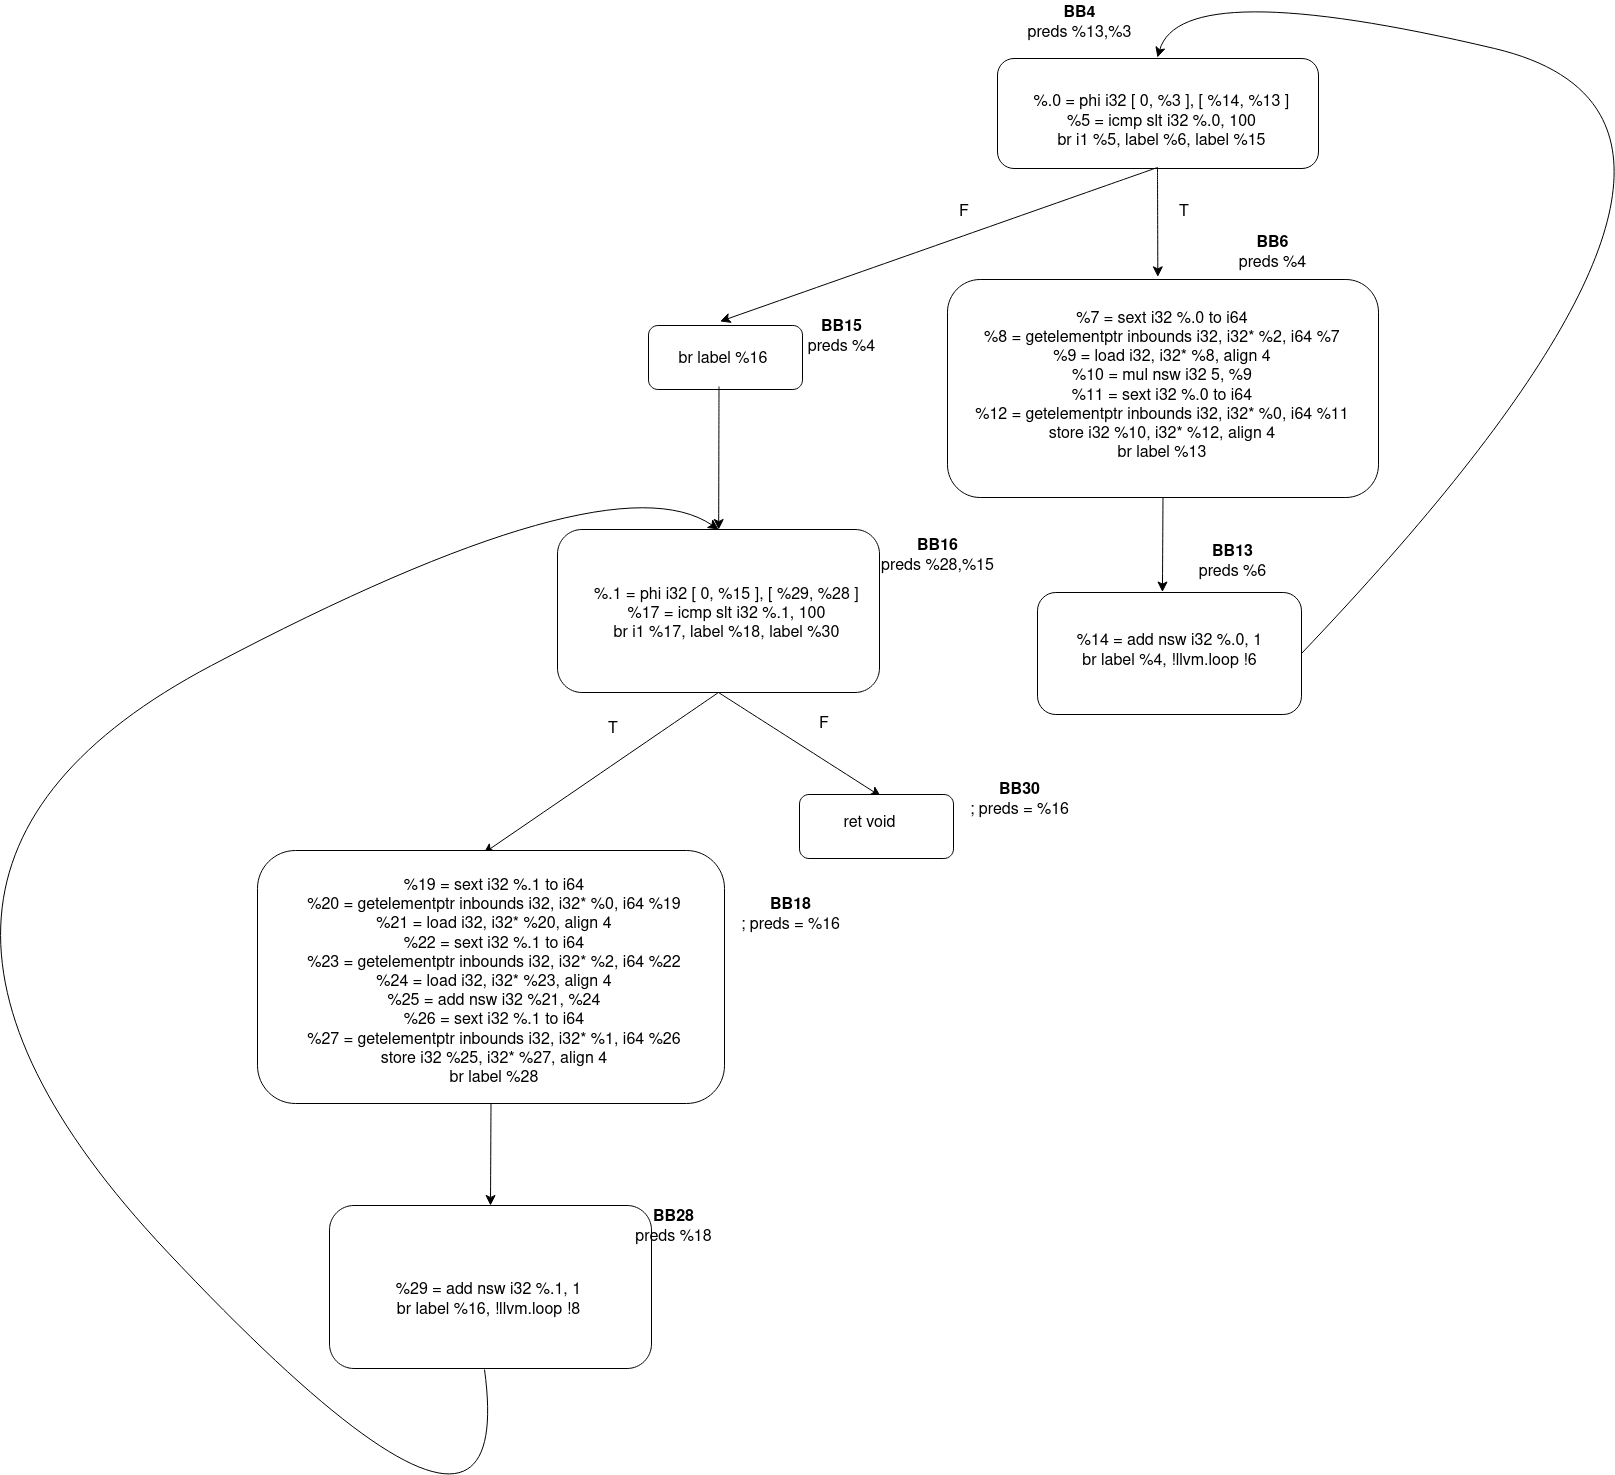
\includegraphics[width=20cm]{./bfore.png}
\caption{CFG prima del passo di ottimizzazione}
\end{figure}

\begin{figure}[H]
\centering
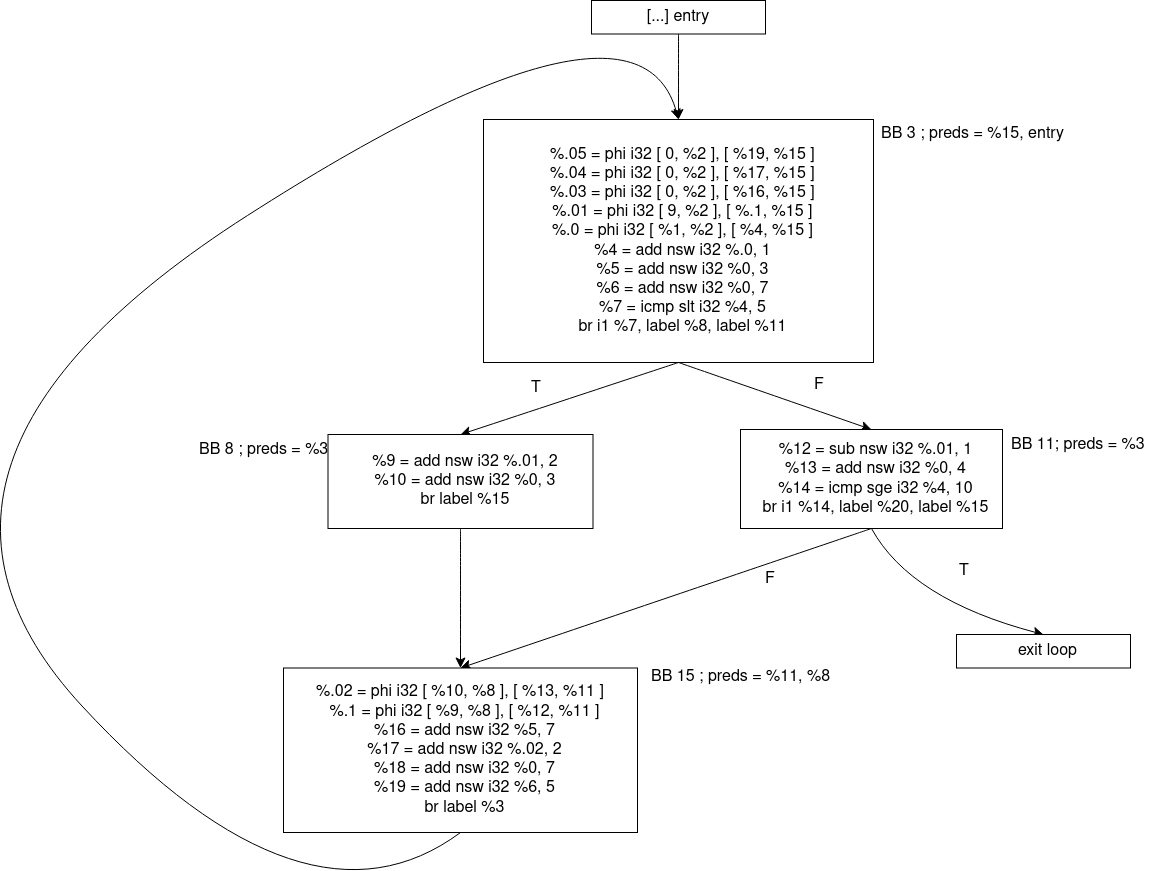
\includegraphics[width=20cm]{./after.png}
\caption{CFG dopo il passo di ottimizzazione}
\end{figure}

\newpage

\begin{multicols}{2}

  \section{Attività sperimentali supplementari}

  Al termine dell'esperienza, si sono poi svolti i seguenti lavori aggiuntivi:

  \begin{itemize}
    \item Confronto delle performance di uno stesso programma, ottimizzato tramite il passo realizzato e non
    \item Sperimentazione volta a determinare la dimensione delle linee di cache sul medesimo calcolatore usato per svolgere l'esperienza
  \end{itemize}

  \subsection{Misura delle performance}
  In primo luogo, si sono ottenuti due file oggetto da \textit{Loop.c}, l'uno servendosi del passo di loop fusion appositamente creato, e l'altro con il comando \textit{llc}, senza fornire particolari flag (dunque non richiedendo esplicitamente ottimizzazioni).\\
  Tali file oggetto sono stati poi linkati in successione ad un semplice script di profiling scritto in C. Il profiler, richiamando la funzione \textit{populate} definita in \textit{Loop.c} in loop esterni per un numero crescente \textit{i} di iterazioni, andava poi a misurare il tempo di esecuzione, per ogni \textit{i}. I valori di \textit{i} sono stati impostati come potenze del 10, per esponente intero $\in [0,9]$.\\

  \begin{figure}[H]
    \centering
    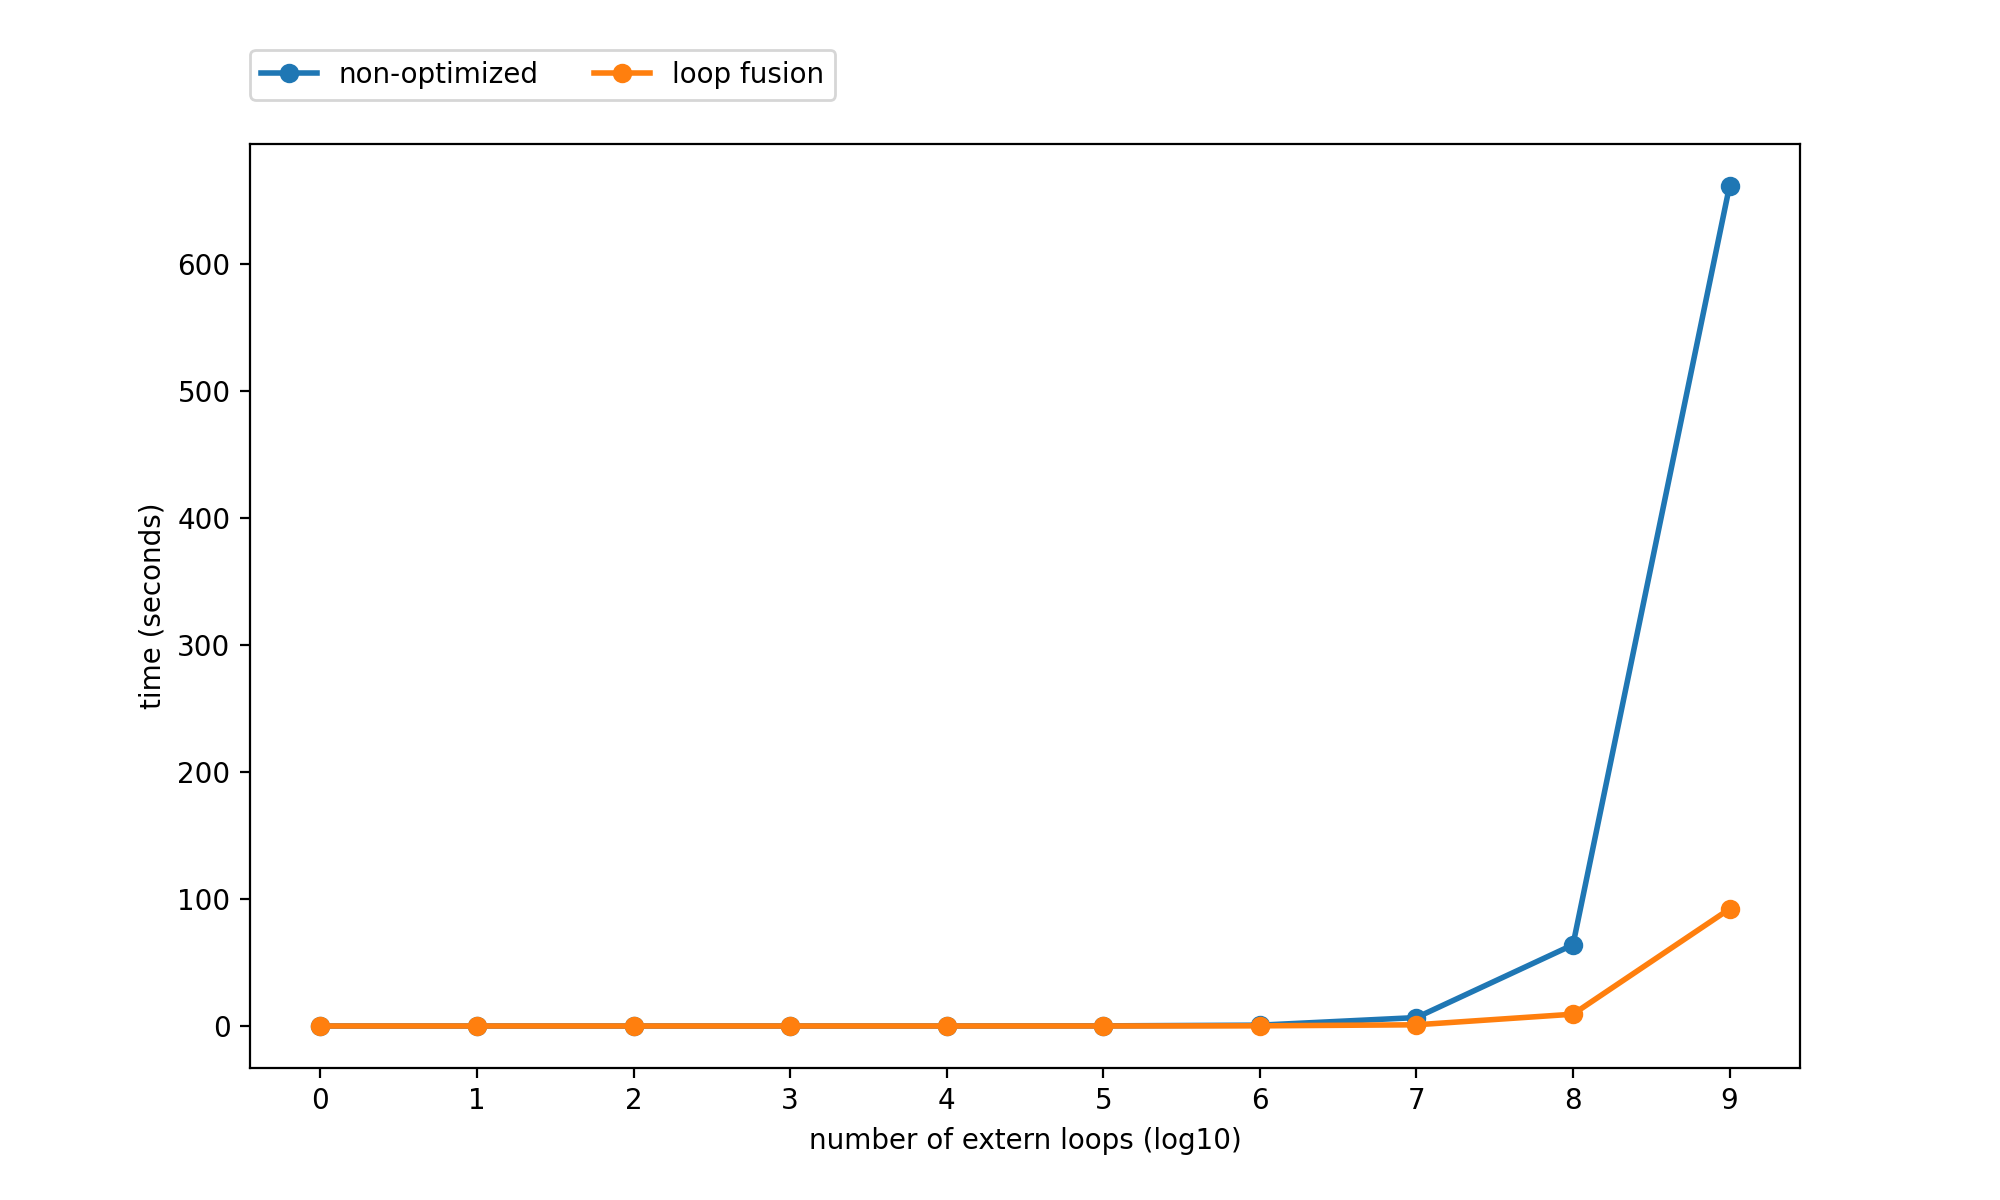
\includegraphics[width = 1.1 \linewidth]{../LocalOpts/graph_1-10.png}
    \caption{Profiling - confronto tra loop fusion e nessun'ottimizzazione, $ODG \in [1,10]$}
  \end{figure}

  Pur essendo chiara la tendenza di miglioramento delle performance nel caso di loop fusion per $i = 10^j, j \in [7, 9], j \in \mathbb{N}$, si è reso necessario verificare l'andamento per valori di \textit{i} più bassi, non visibile di fatto su quest'ultimo grafico.

  \begin{figure}[H]
    \centering
    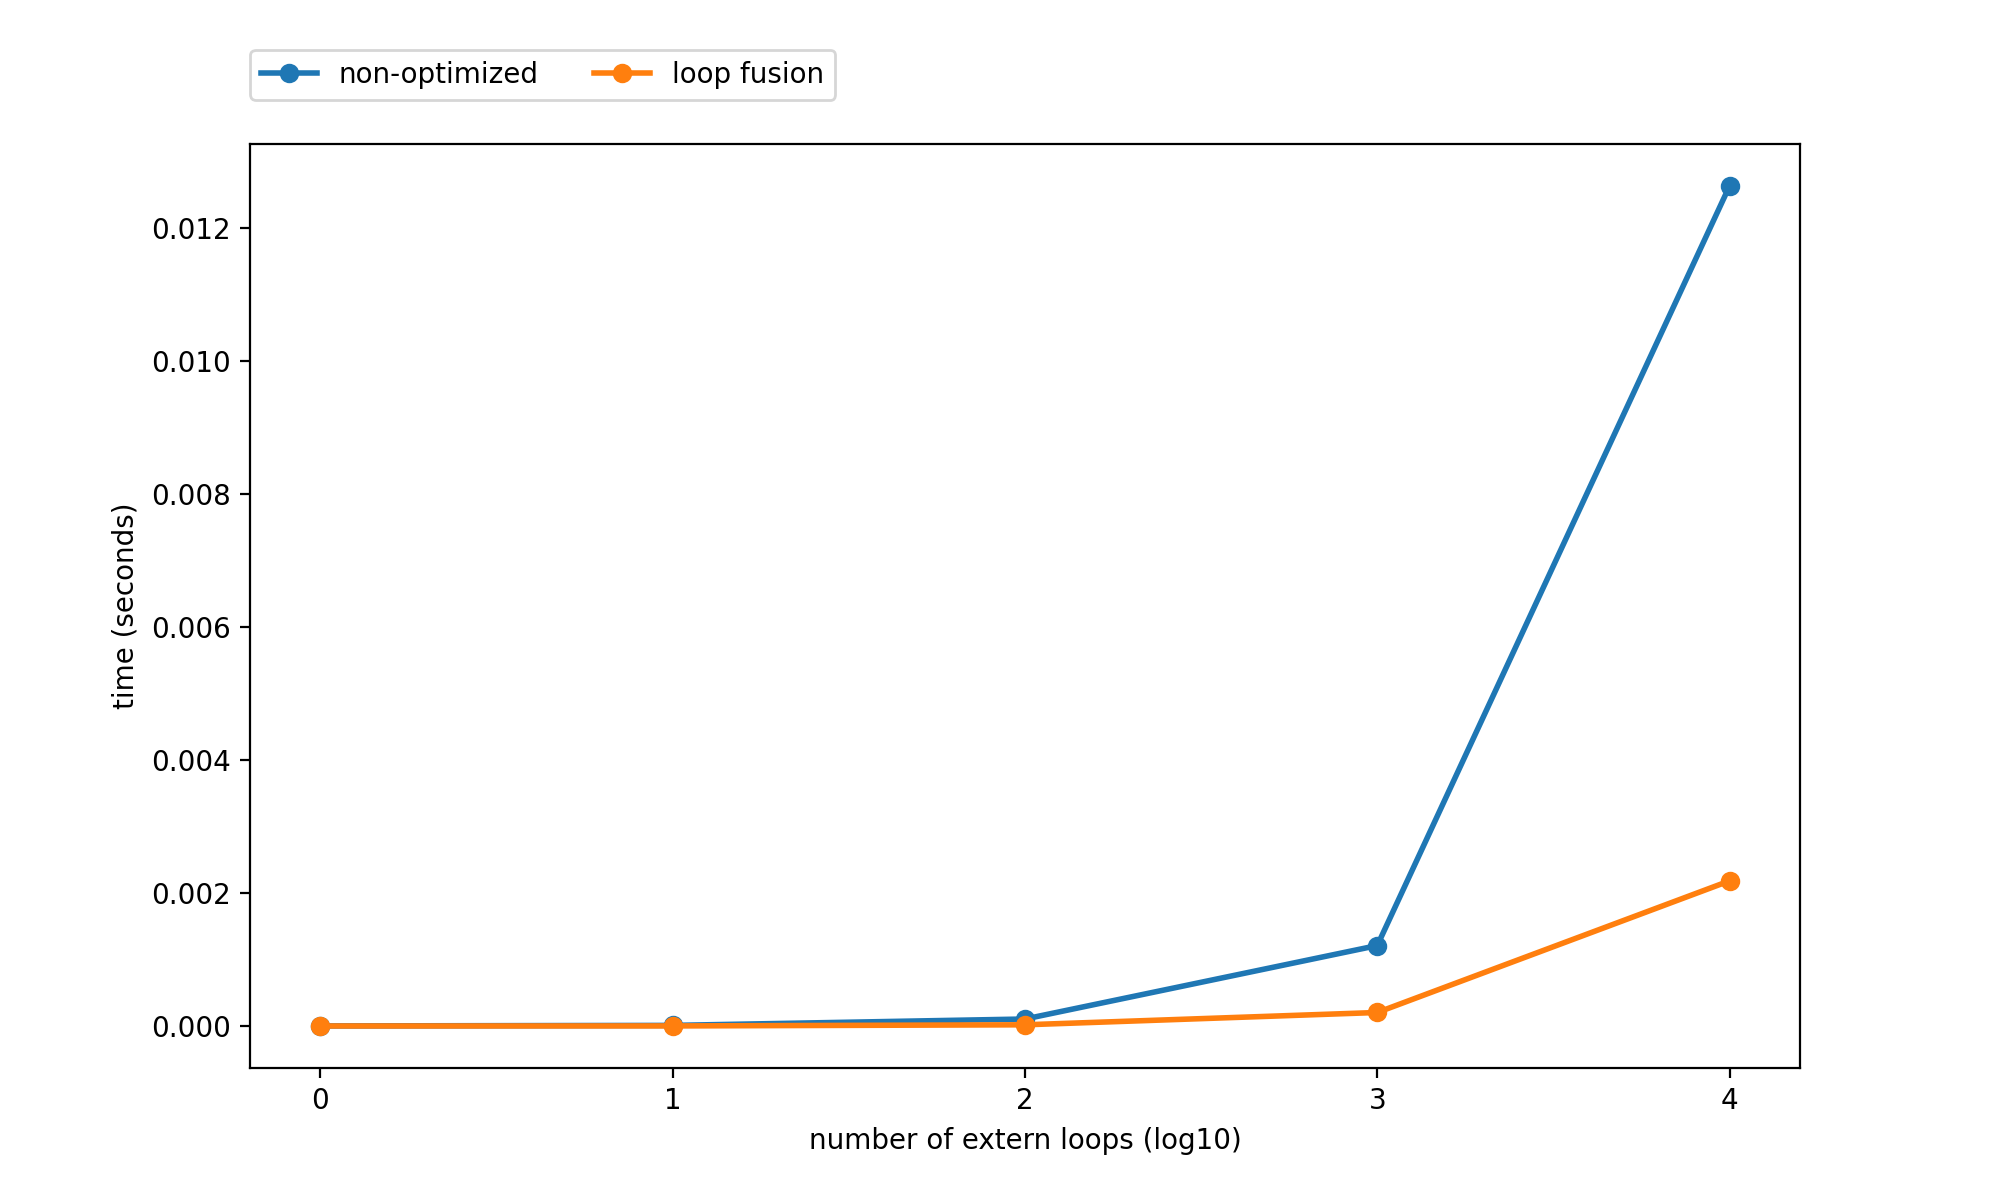
\includegraphics[width = 1.1 \linewidth]{../LocalOpts/graph_1-5.png}
    \caption{Profiling - confronto tra loop fusion e nessun'ottimizzazione, $ODG \in [1,5]$}
  \end{figure}

  Infine, si è osservato il comportamento del profiler tra i primi 3 ordini di grandezza, confermando quanto già visto.

  \begin{figure}[H]
    \centering
    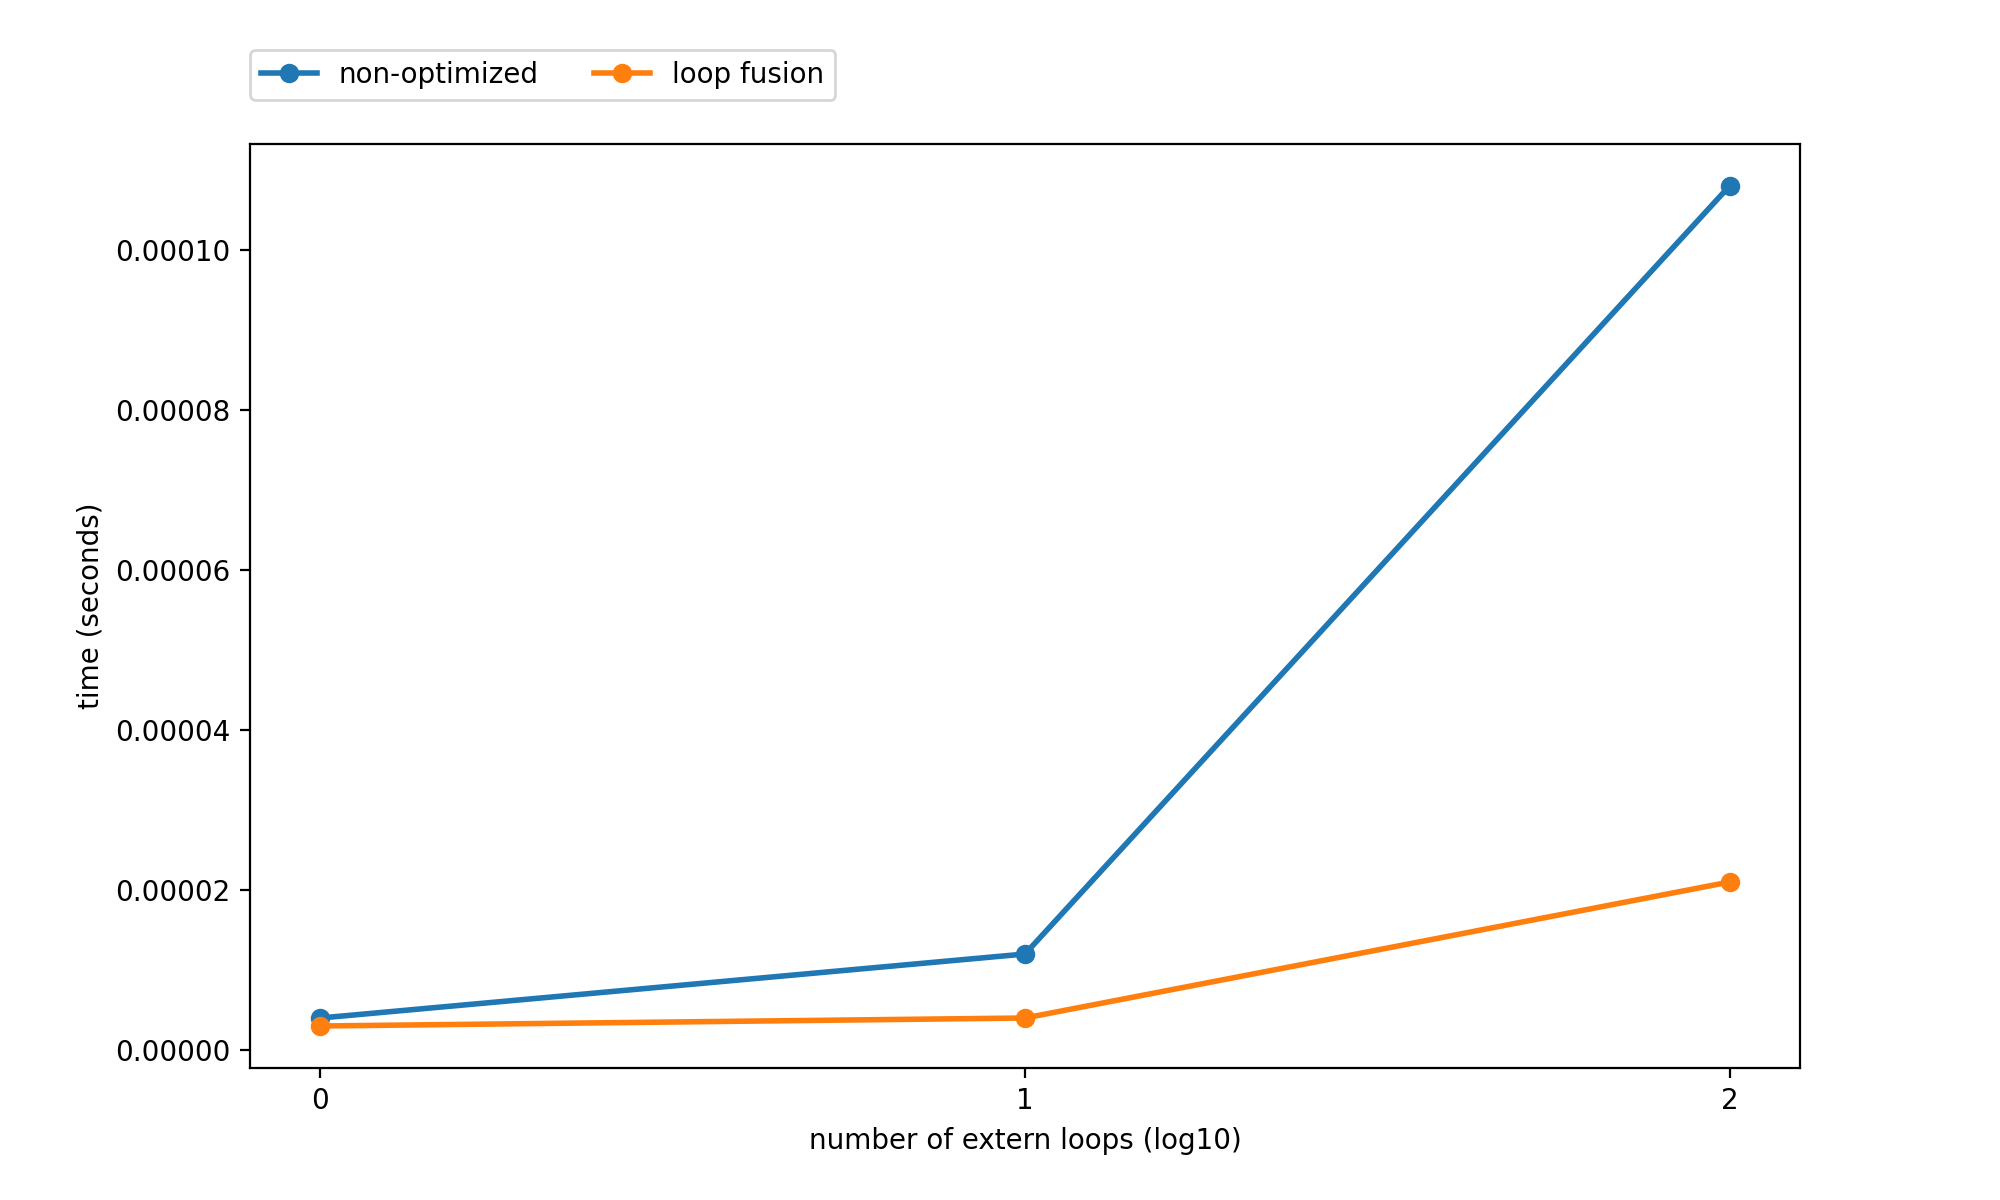
\includegraphics[width = 1.1 \linewidth]{../LocalOpts/graph_1-3.png}
    \caption{Profiling - confronto tra loop fusion e nessun'ottimizzazione, $ODG \in [1,3]$}
  \end{figure}

  Il tempo di esecuzione ha una tenenza di crescita esponenziale per entrambe le linee. Si è quindi deciso di eseguire un ulteriore plot, riportando sull'asse \textit{y} il logaritmo del tempo di esecuzione, per meglio osservare il rapporto tra i tempi di esecuzione ad uguali valori di \textit{i}.

  \begin{figure}[H]
    \centering
    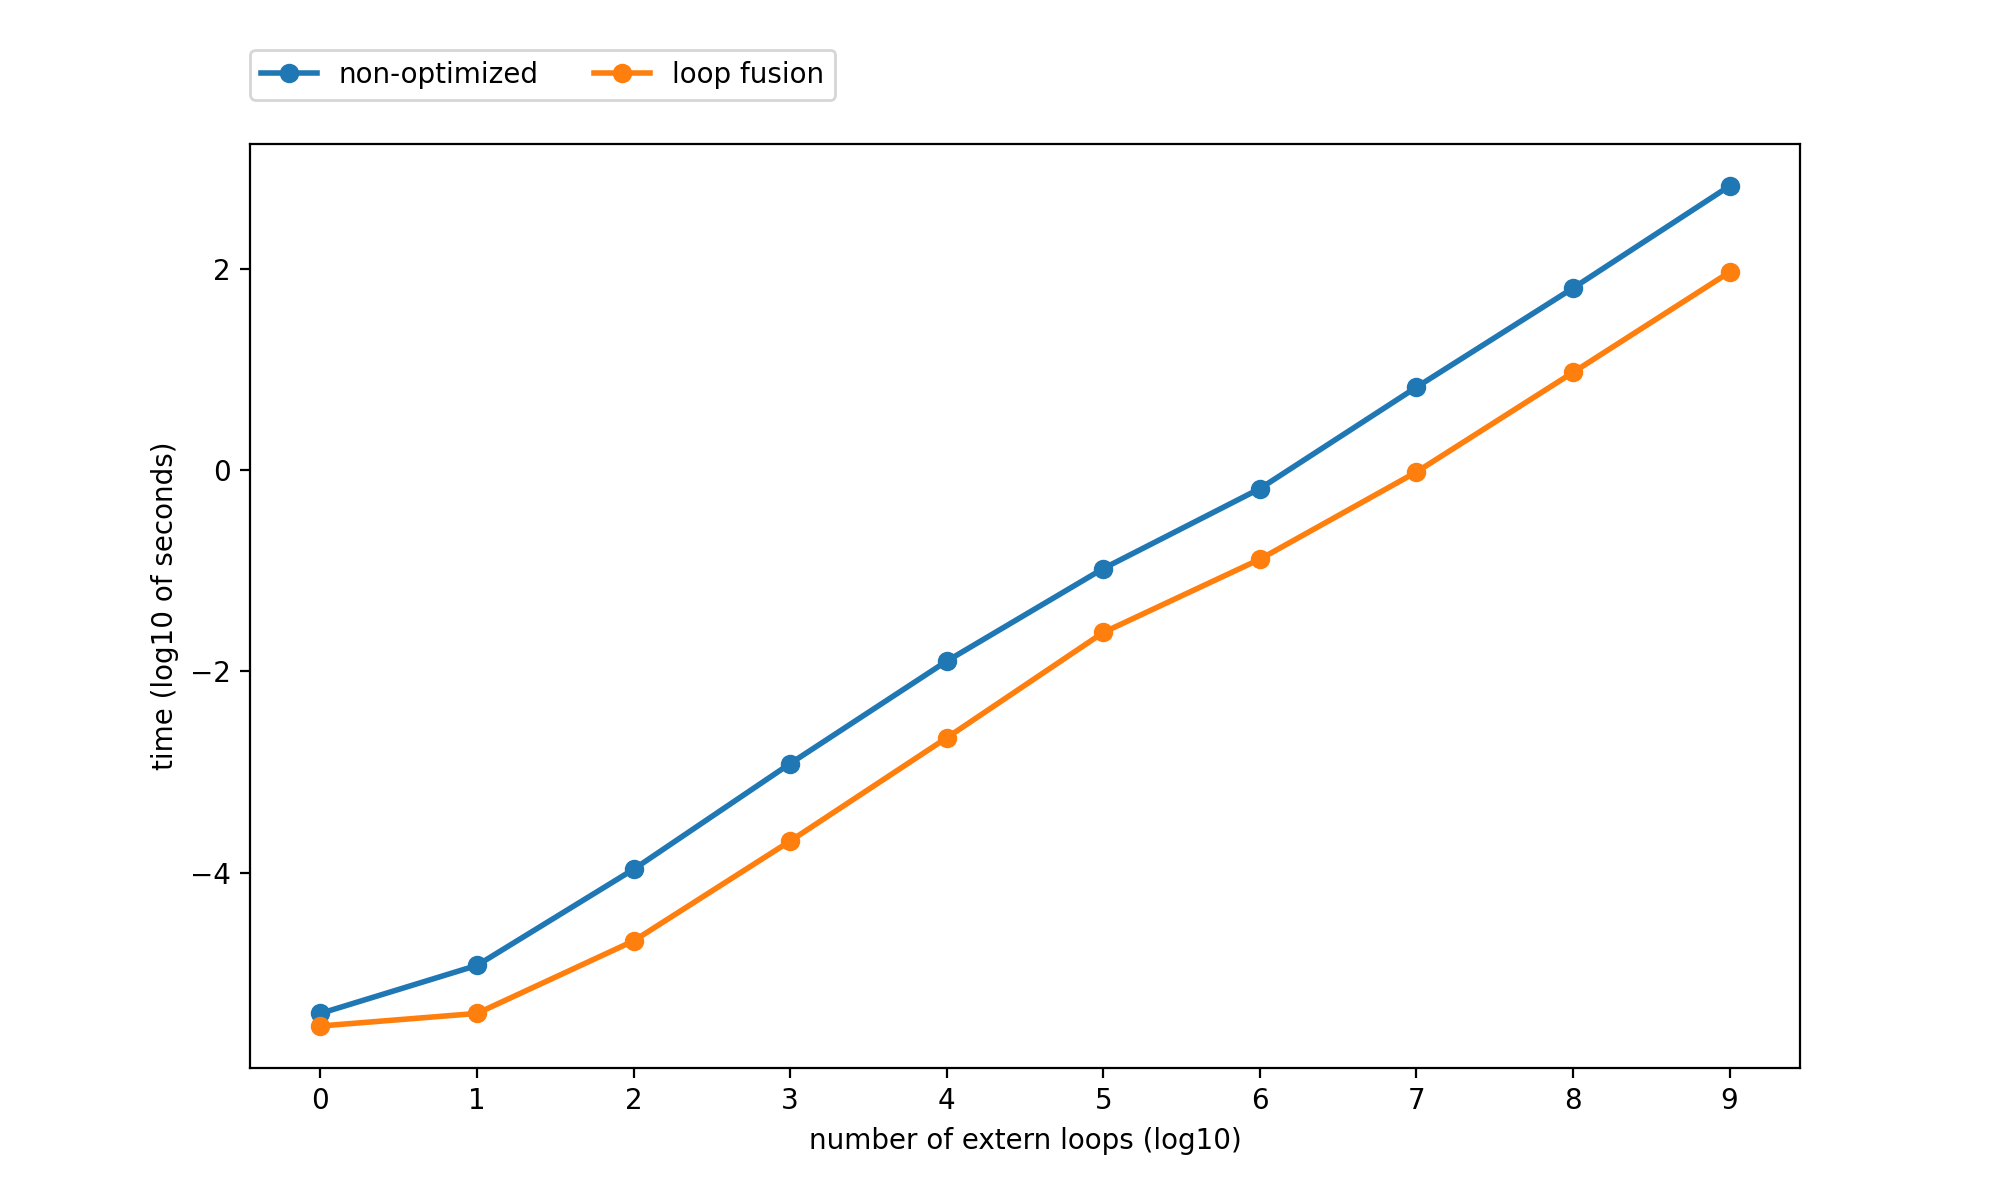
\includegraphics[width = 1.1 \linewidth]{../LocalOpts/graph_log.png}
    \caption{Profiling - confronto tra loop fusion e nessun'ottimizzazione, $\log_{10}{t}$ su asse \textit{y}}
  \end{figure}

  Dopo un iniziale assestamento, ed al crescere di \textit{i}, il rapporto tra le prestazioni con e senza loop fusion si conserva circa stabile (esecuzione $\sim 5-7$ volte più rapida con loop fusion).

\end{multicols}

\end{document}
